%% 美赛模板:正文部分

\documentclass[12pt]{article}  % 官方要求字号不小于 12 号,此处选择 12 号字体

% 本模板不需要填写年份,以当前电脑时间自动生成
% 请在以下的方括号中填写队伍控制号
\usepackage[2306372]{easymcm}  % 载入 EasyMCM 模板文件
\problem{C}  % 请在此处填写题号
\usepackage{mathptmx}  % 这是 Times 字体,中规中矩 
%\usepackage{mathpazo}  % 这是 COMAP 官方杂志采用的更好看的 Palatino 字体,可替代以上的 mathptmx 宏包

\title{An MCM Paper Made by Team 2306372}  % 标题

% 如需要修改题头(默认为 MCM/ICM),请使用以下命令(此处修改为 MCM)
%\renewcommand{\contest}{MCM}

% 文档开始
\begin{document}

% 此处填写摘要内容
\begin{abstract}
In today's society, the game industry is booming and more and more people are participating in the game industry. Games have become part of everyone's life.So many games are so well made and so expensive that games are now known as the Ninth art.The wordle this game, only five letters, simple game six speculation has attracted millions of people visit, hundreds of thousands of twitter to share every day.The popularity of the game has also attracted the attention of all sectors of society. The New York Times invited us to build a model to predict how the number of Wordle users changes and how word attributes influence the number of guesses and accuracy of users.At the beginning, our team thought that the first question was very simple. We used simple exponential fitting and Gaussian fitting to complete the first question to predict the number of people on March 1st, and the fitting effect was very good. The number of people predicted by the index on March 1 was 18,785, and the goodness of fit 
$R^2 = 0.9968$. 
The number of people predicted by the index on March 1 was 13,914, and the goodness of fit 
$R^2 = 0.9892$.
But we later found out that all of the data was shared by Twitter users and not by all of the players. The idea of survivor bias immediately came to mind.Immediately decided to optimize their own models.


    % 美赛论文中无需注明关键字。若您一定要使用,
    % 请将以下两行的注释号 '%' 去除,以使其生效
    % \vspace{5pt}
    % \textbf{Keywords}: MATLAB, mathematics, LaTeX.

\end{abstract}

\maketitle  % 生成 Summary Sheet
\tableofcontents  % 生成目录


% 正文开始
\section{Introduction}
\subsection{Problem Background}
The New York Times wordle game was born. The simple five-letter, six-guess game rules aroused wide attention of the society. And the effect of the attributes of the word on the result of the guess got us thinking. After a cursory search, we found that there are as many as 30,000 five-letter English words, and they cover all aspects of life. The inexhaustible question bank brings new game experiences for everyone. By analyzing the attributes of a word, we can rate the words and identify their difficulty. To better predict how the public will play wordle in the future.


Two major problems are discussed in this paper, which are:
\begin{itemize}
     \item What are the attributes of a five-letter word.
    \item Complete the specific and practical word rating program and analyze the difficulty coefficient of five-letter words.
\end{itemize}

\subsection{Literature Review}
A literatrue\cite{1} say something about this problem ...

\subsection{Our work}
We do such things ...

\begin{enumerate}[\bfseries 1.]
    \item We do ...
    \item We do ...
    \item We do ...
\end{enumerate}

\section{Preparation of the Models}
\subsection{Assumptions}

\subsection{Notations}
The primary notations used in this paper are listed in Table \ref{tb:notation}.



\section{The Models}
\subsection{Model 1}
\subsubsection{Exp prediction and Gaussian prediction}
The detail can be described by equation :

\begin{equation}
\large f(x)=a\cdot  e^{bx}+c\cdot e^{dx}
\end{equation}

$$Coefficient(Confidence \quad bounds: 95\%)$$
\begin{table}[!htbp]
	\begin{center}
		\caption{Exp prediction}
		\begin{tabular}{cl}
			\toprule
			\multicolumn{1}{m{3cm}}{\centering Formula}
			&\multicolumn{1}{m{8cm}}{\centering Range}\\
			\midrule
			$a=7.07e+05$&   \qquad\qquad (6.83e+05, 7.309e+05)\\
			$b=-0.02465$&   \qquad\qquad (-0.02556, -0.02375)\\
			$ c=6.184e+04$ &  \qquad\qquad  (5.503e+04, 6.864e+04)\\
			\bottomrule
		\end{tabular}\label{tb:notation}
	\end{center}
\end{table}

\begin{equation}
\large f(x) =  a_1\cdot e^{-\frac{x-b_1}{c_1}^2} + a_2\cdot e^{-\frac{x-b_2}{c_2}^2}
\end{equation}

$$Coefficient(Confidence bounds: 95\%)$$

\begin{table}[!htbp]
	\begin{center}
		\caption{Gauss prediction}
		\begin{tabular}{cl}
			\toprule
			\multicolumn{1}{m{3cm}}{\centering Formula}
			&\multicolumn{1}{m{8cm}}{\centering Range}\\
			\midrule
			$a1 =  1.014e+18 $&   \qquad\qquad(-7.45e+20, 7.47e+20)\\
			$b1 =  -2997$&   \qquad\qquad (-8.057e+04, 7.457e+04)\\
			$c1 =  565.3$ &  \qquad\qquad  (-6672, 7803)\\
			$a2 =  2.748e+04$&   \qquad\qquad (6742, 4.822e+04)\\
			$b2 =  244 $&   \qquad\qquad (34.64, 453.3)\\
			$c2 =  210.6$ &  \qquad\qquad  (-14.9, 436.1)\\
			\bottomrule
		\end{tabular}\label{tb:notation}
	\end{center}
\end{table}



\begin{figure}[htbp]
	
	\begin{subfigure}[b]{.5\textwidth}
		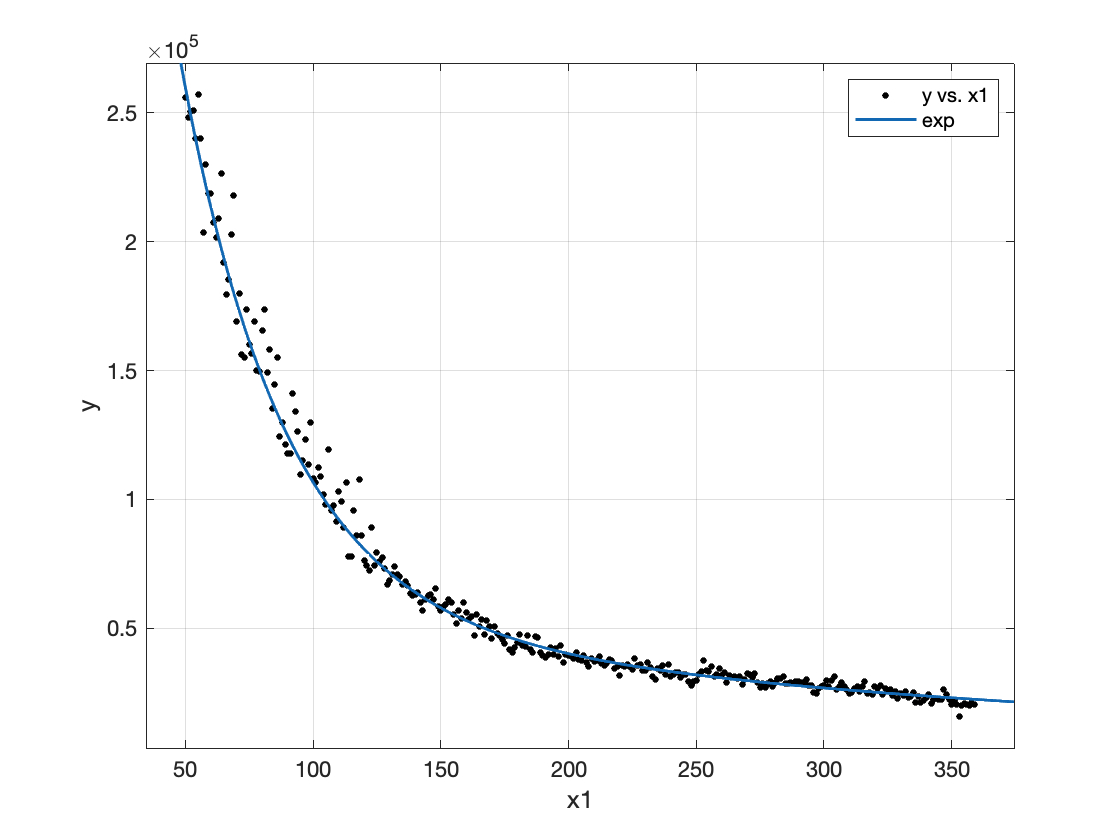
\includegraphics[width=\textwidth]{exp.jpg}
		\caption{Exp prediction}\label{subfig:left}
	\end{subfigure}
	\begin{subfigure}[b]{.5\textwidth}
		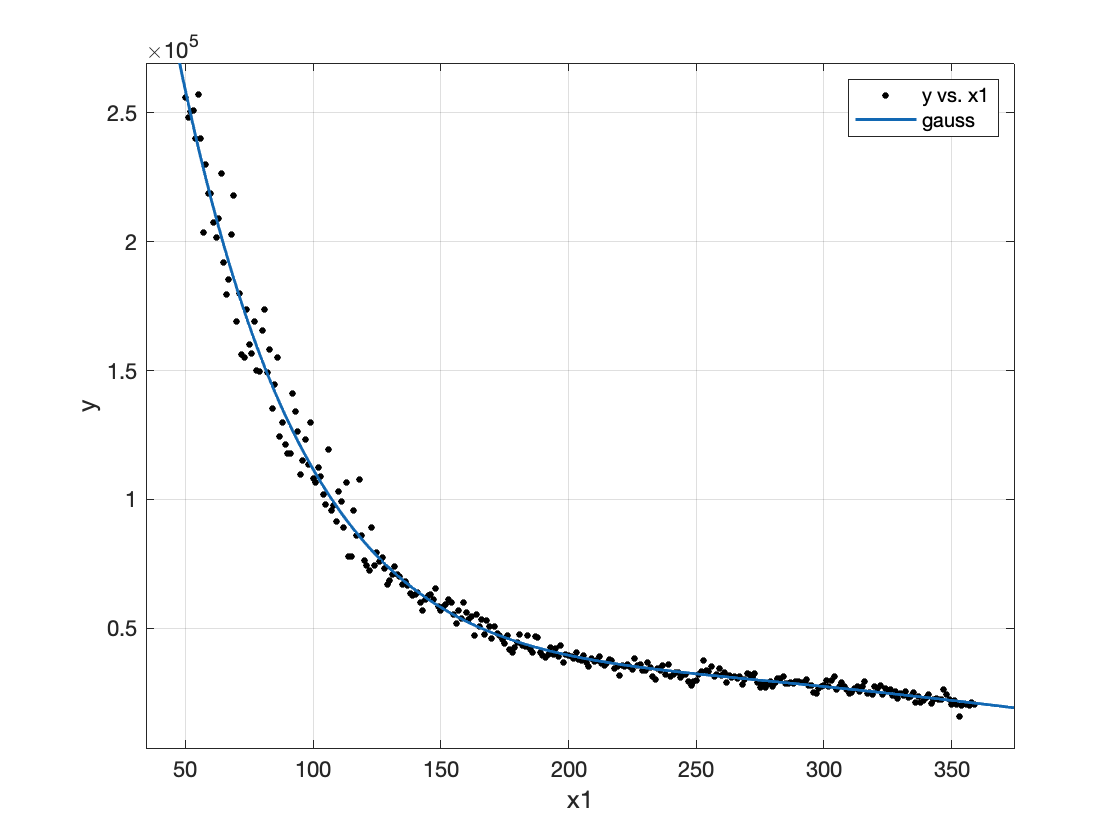
\includegraphics[width=\textwidth]{gauss.jpg}
		\caption{Gaussian predicition}\label{subfig:right}
	\end{subfigure}
	\caption{{The outcome }\label{fig:subfigures}
	\end{figure}






\subsection{Model 2}
\subsubsection{Conclusion of Model 2}
The results are shown in Figure \ref{fig:result}, where $t$ denotes the time in seconds, and $c$ refers to the concentration of water in the boiler.

\subsection{Model 3}
\subsubsection{Conclusion of Model 3}
The results are shown in Figure \ref{fig:result}, where $t$ denotes the time in seconds, and $c$ refers to the concentration of water in the boiler.

\begin{figure}[htbp]
\centering
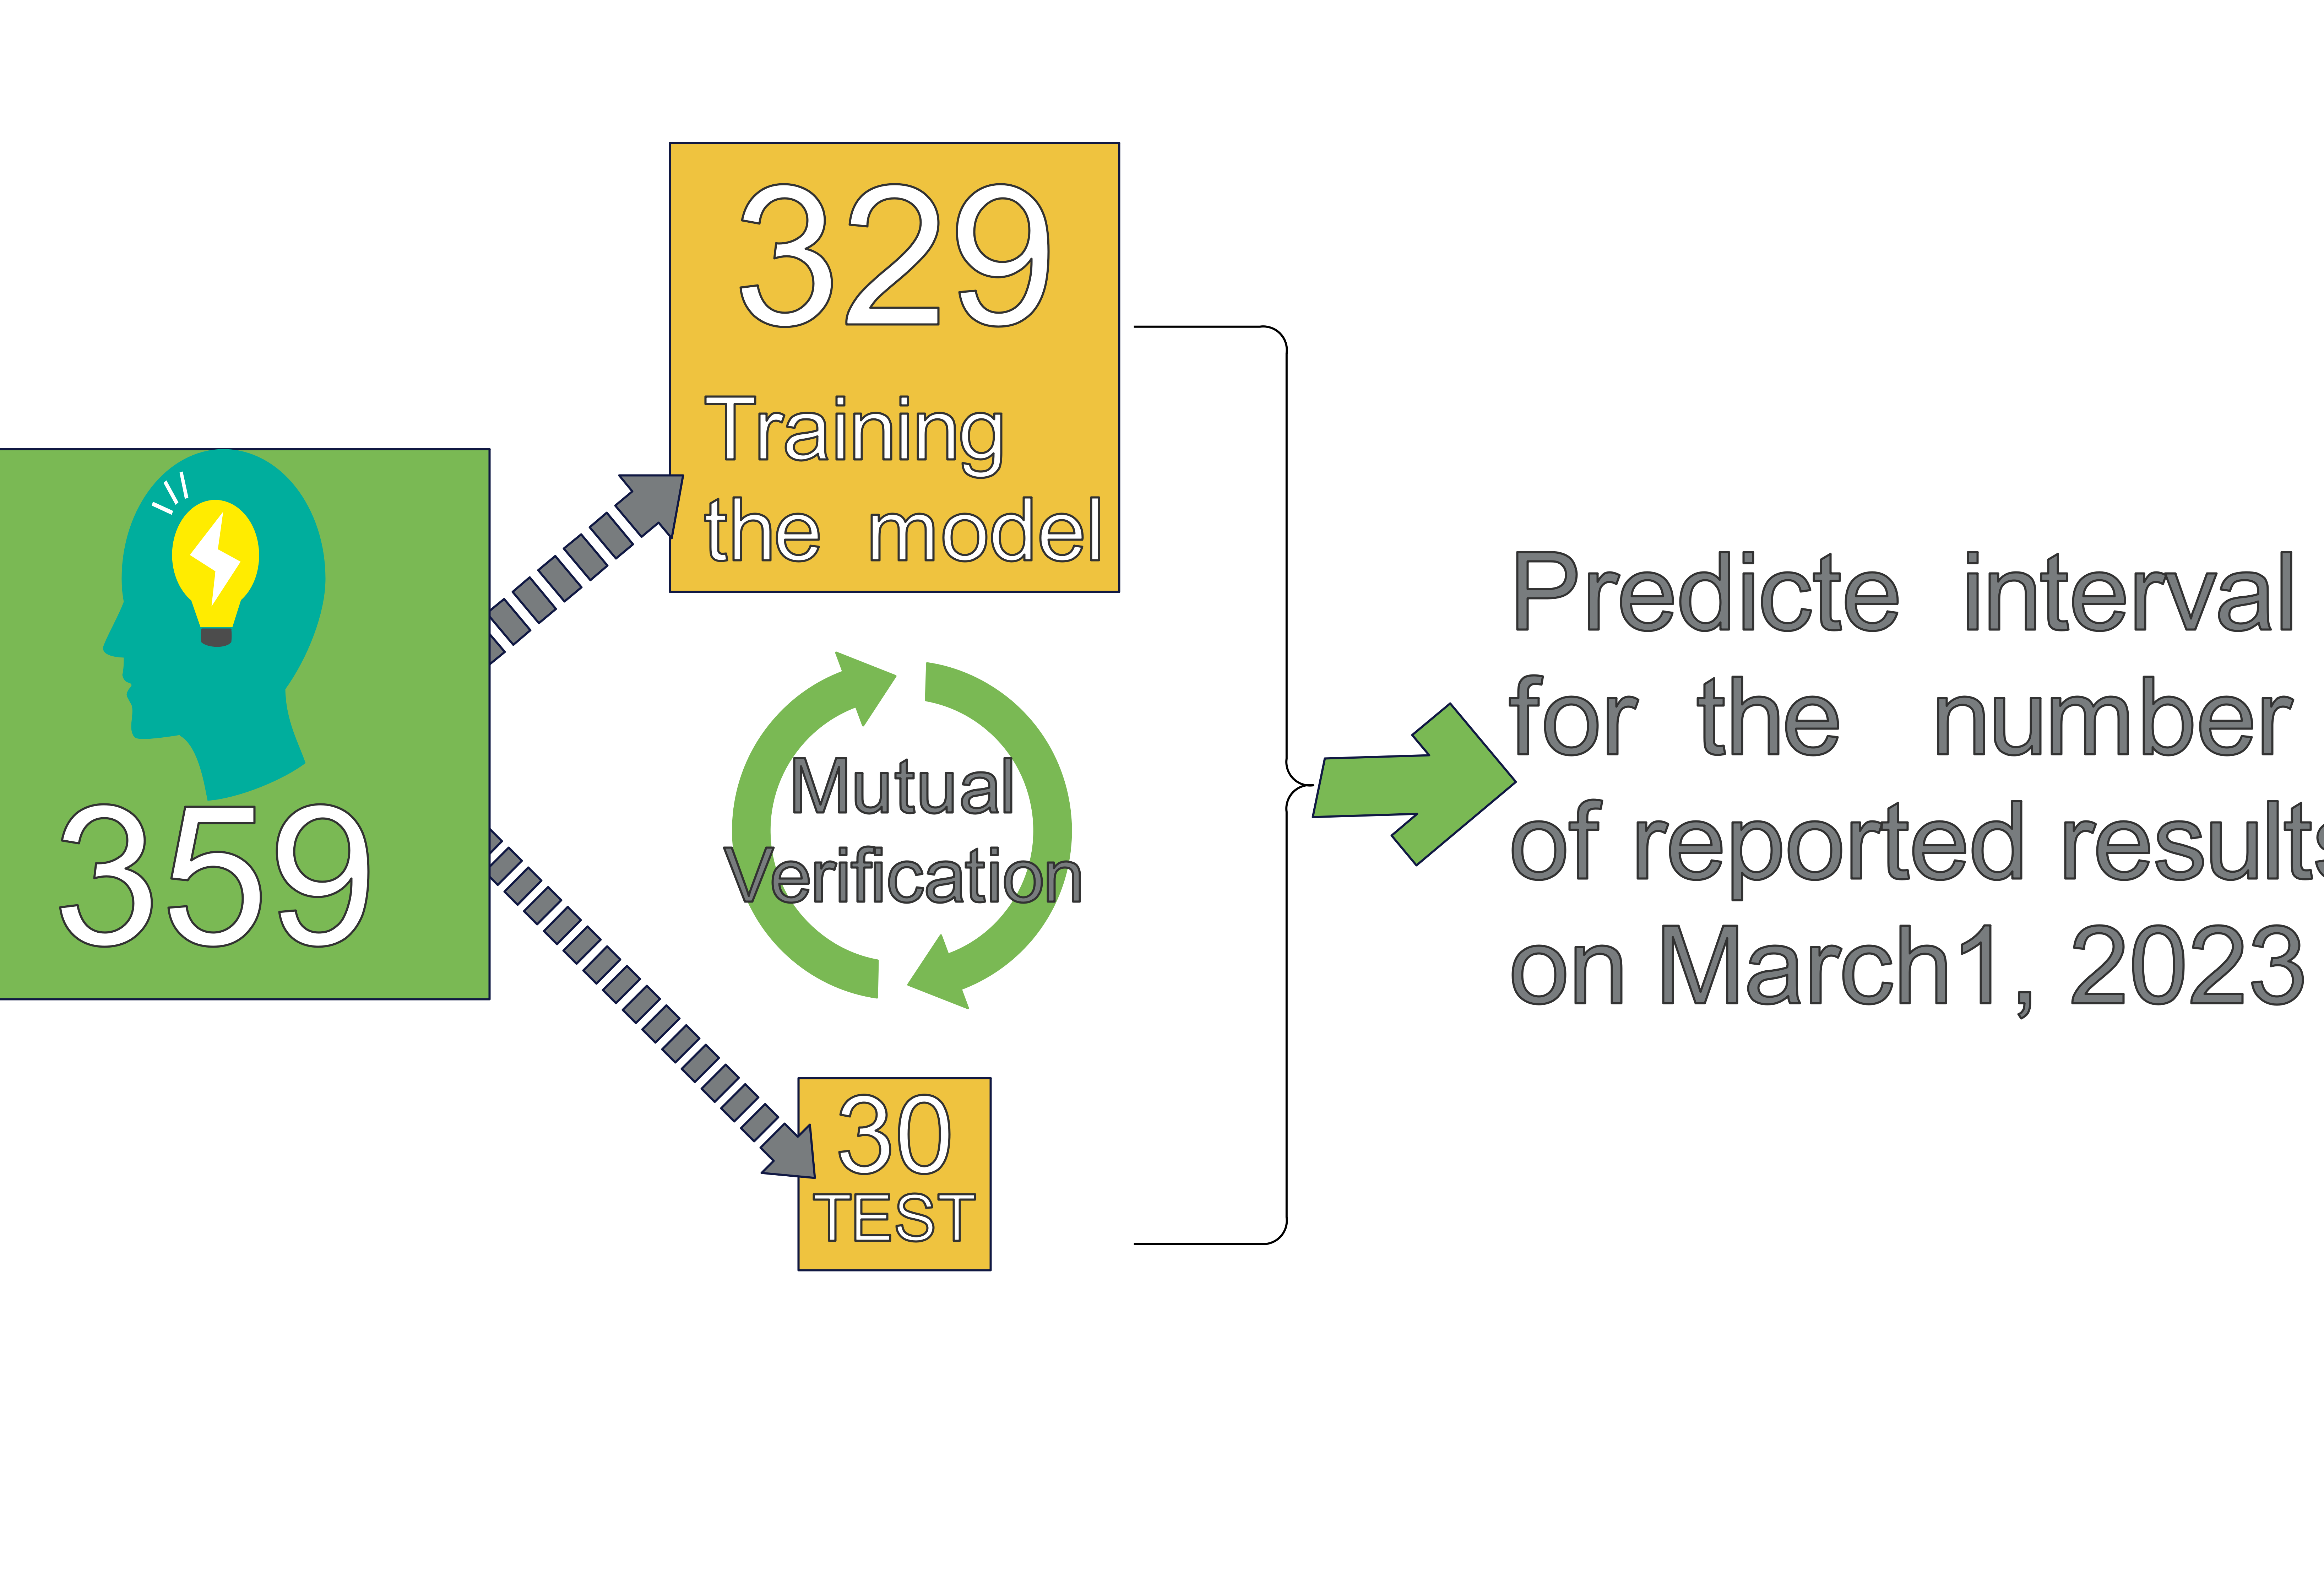
\includegraphics[width=.9\textwidth]{March.png}
\caption{The number of reported result on March 1,2023}\label{fig:result}
\end{figure}

\begin{figure}[htbp]
	\centering
	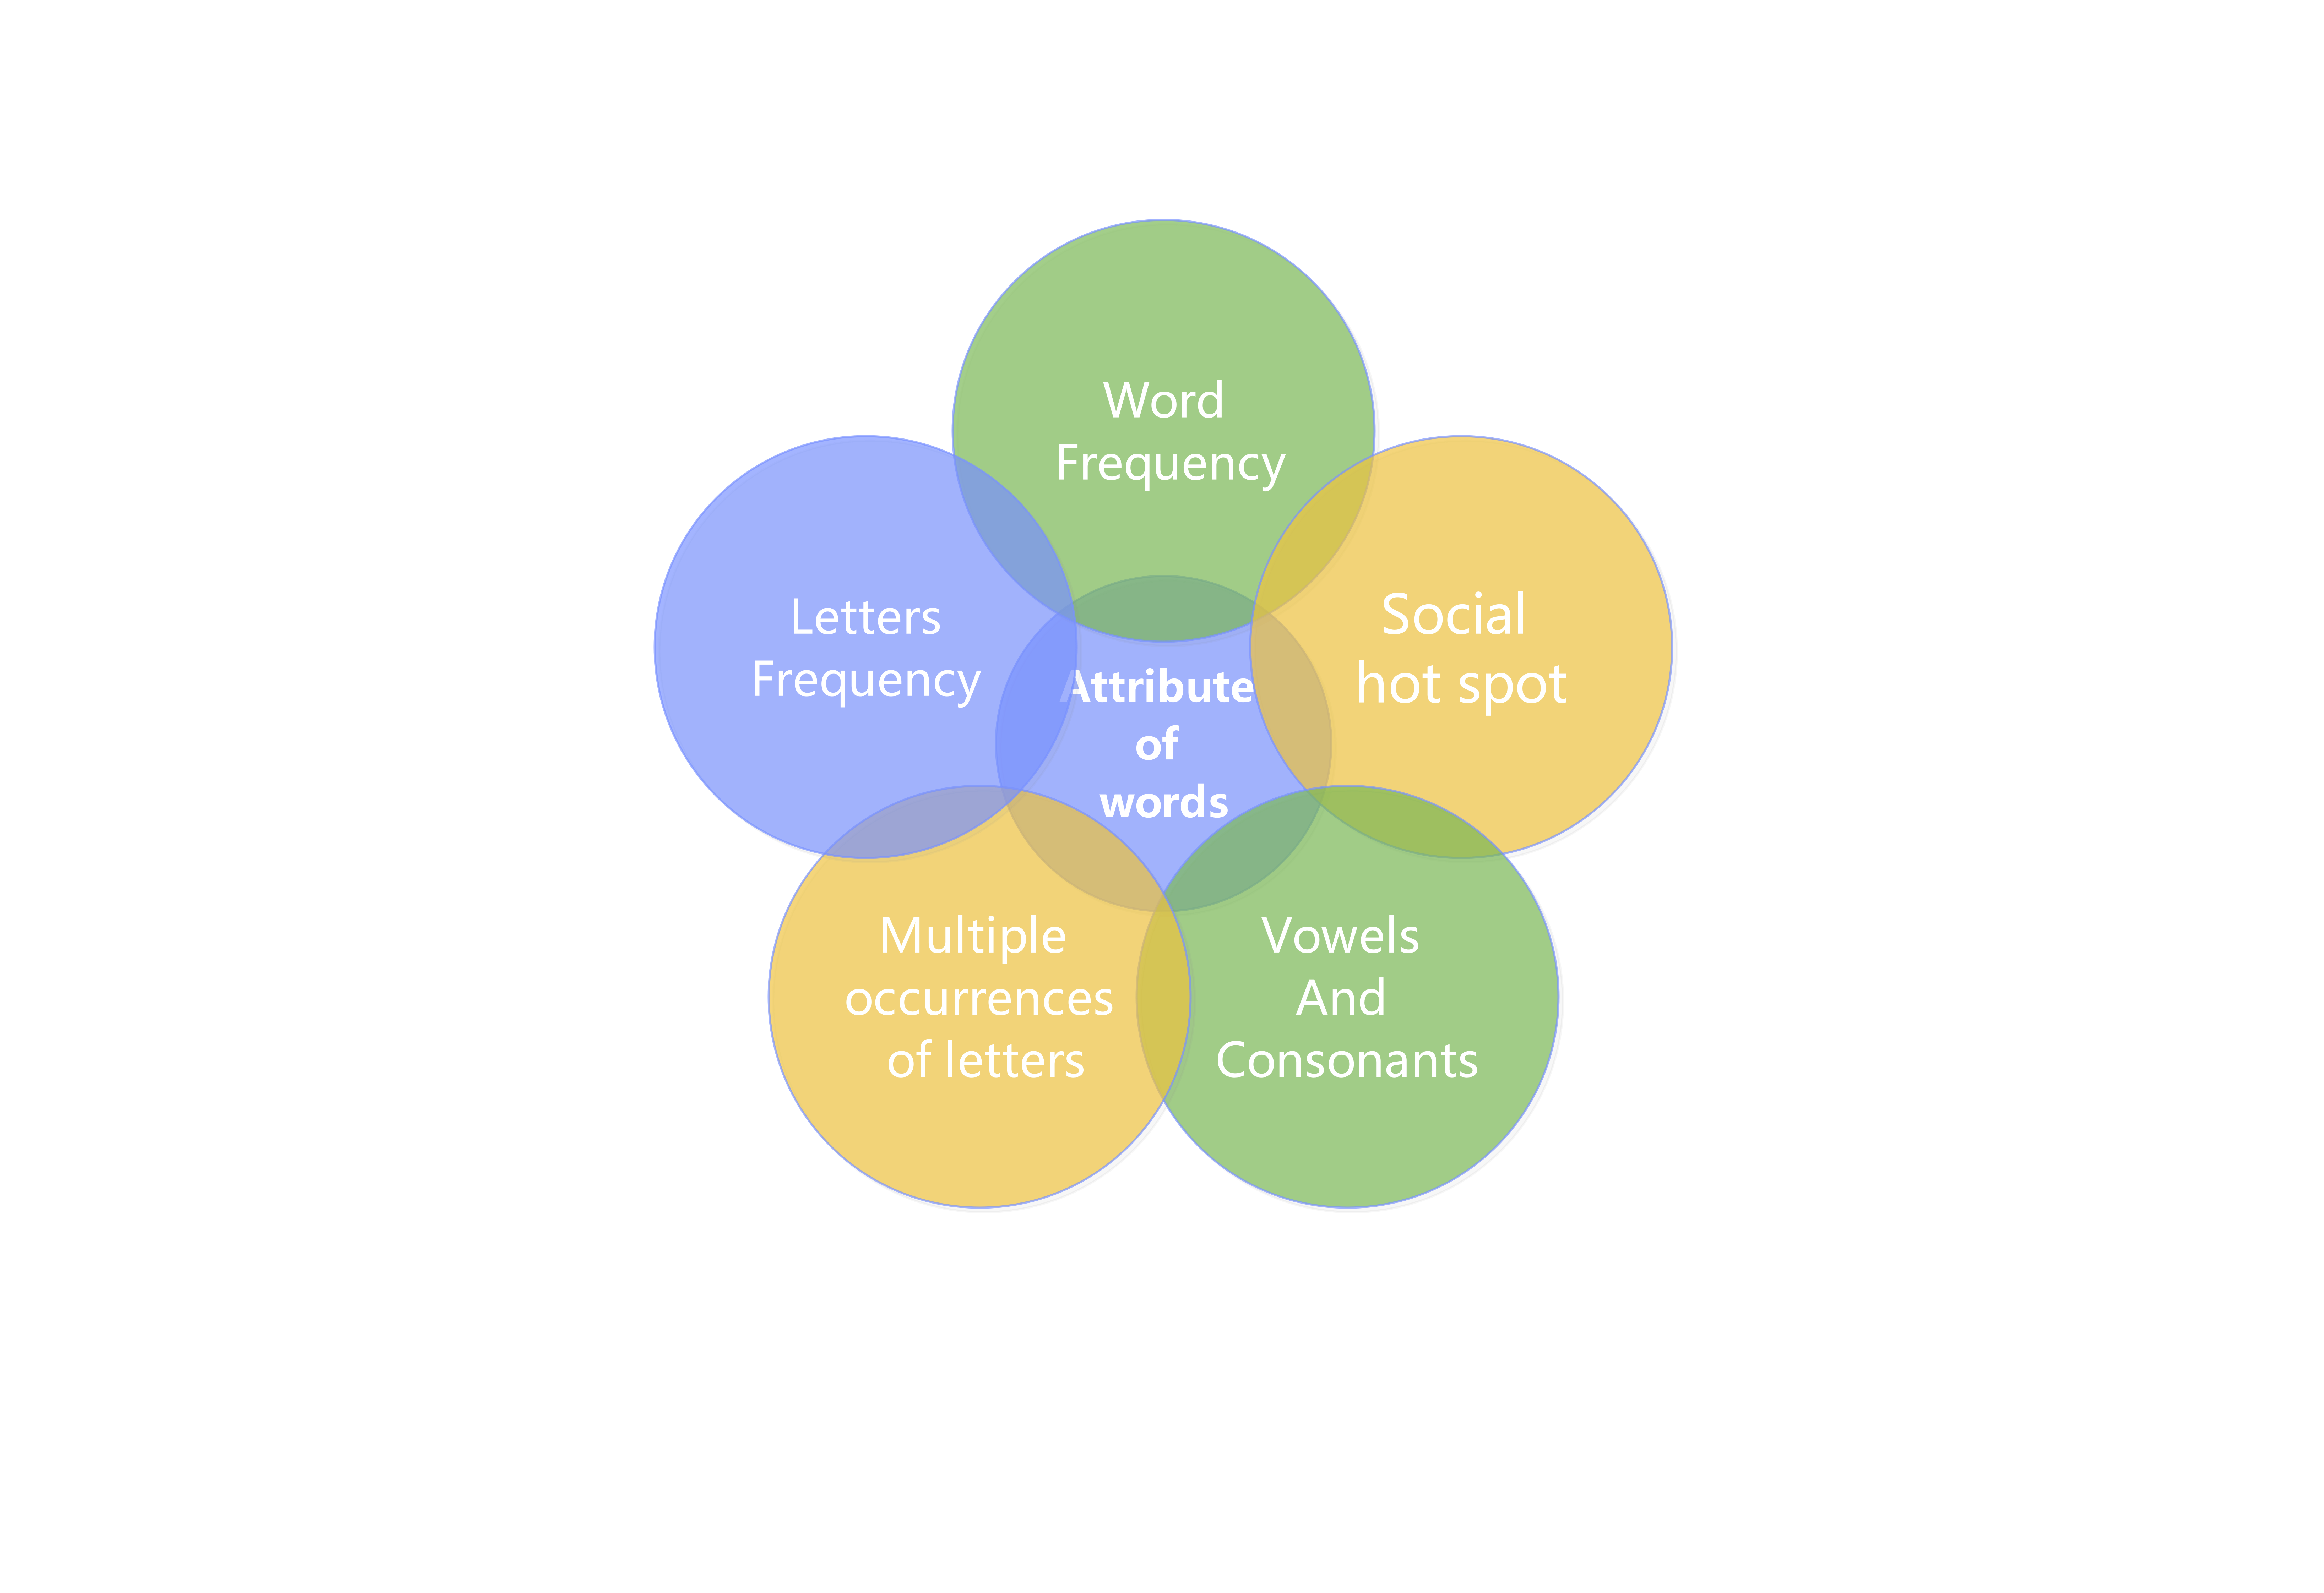
\includegraphics[width=0.9\textwidth]{attribute.png}
	\caption{The attritube of words}\label{fig:result}
\end{figure}


\clearpage
\subsubsection{Commetary on Model 3}
The instance of long and wide tables are shown in Table \ref{tb:longtable}.

% 长表格示例,更多用法请参考 longtable 宏包文档
% 以下环境及对应参数可实现表格内的自动换行与表格的自动断页
% 您也可以选择自行载入 tabularx 宏包,并通过 X 参数指定对应列自动换行
\begin{longtable}{ p{4em} p{14em} p{14em} }
\caption{Basic Information about Three Main Continents (scratched from Wikipedia)}
\label{tb:longtable}\\
\toprule
Continent & Description & Information \\
\midrule
Africa & Africa Continent is surrounded by the Mediterranean Sea to the
north, the Isthmus of Suez and the Red Sea to the northeast, the Indian
Ocean to the southeast and the Atlantic Ocean to the west. &
At about 30.3 million km$^2$ including adjacent islands, it covers 6\%
of Earth's total surface area and 20\% of its land area. With 1.3
billion people as of 2018, it accounts for about 16\% of the world's
human population. \\
\midrule
Asia & Asia is Earth's largest and most populous continent which
located primarily in the Eastern and Northern Hemispheres.
It shares the continental landmass of Eurasia with the continent
of Europe and the continental landmass of Afro-Eurasia with both
Europe and Africa. &
Asia covers an area of 44,579,000 square kilometres, about 30\%
of Earth's total land area and 8.7\% of the Earth's total surface
area. Its 4.5 billion people (as of June 2019) constitute roughly
60\% of the world's population. \\
\midrule
Europe & Europe is a continent located entirely in the Northern
Hemisphere and mostly in the Eastern Hemisphere. It comprises the
westernmost part of Eurasia and is bordered by the Arctic Ocean to
the north, the Atlantic Ocean to the west, the Mediterranean Sea to
the south, and Asia to the east. &
Europe covers about 10,180,000 km$^2$, or 2\% of the Earth's surface
(6.8\% of land area), making it the second smallest
continent. Europe had a total population of about 741 million (about
11\% of the world population) as of 2018. \\
\bottomrule

\end{longtable}

Figure \ref{fig:subfigures} gives an example of subfigures. Figure \ref{subfig:left} is on the left, and Figure \ref{subfig:right} is on the right.

% 子图(多图并列)示例,更多用法请参考 subfigure 宏包文档
% 如果您只希望几张图并列,不需要额外的 caption,那么在 figure 环境中
% 连续插入总宽度不超过 \textwidth 的多个 \includegraphics 命令即可
\begin{figure}[htbp]
\centering
\begin{subfigure}[b]{.4\textwidth}
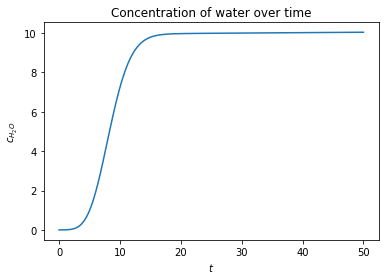
\includegraphics[width=\textwidth]{water.png}
\caption{Image on the left}\label{subfig:left}
\end{subfigure}
\begin{subfigure}[b]{.4\textwidth}
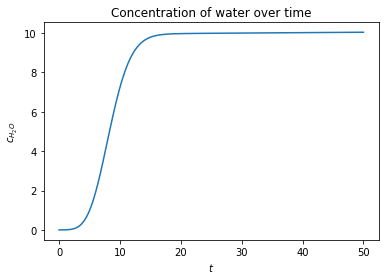
\includegraphics[width=\textwidth]{water.png}
\caption{Image on the right}\label{subfig:right}
\end{subfigure}
\caption{Two images}\label{fig:subfigures}
\end{figure}

\section{Strengths and Weaknesses}
\subsection{Strengths}
\begin{itemize}
    \item First one...
    \item Second one ...
\end{itemize}

\subsection{Weaknesses}
\begin{itemize}
    \item Only one ...
 \end{itemize}


% 以下为信件/备忘录部分,不需要可自行去掉
% 如有需要可将整个 letter 环境移动到文章开头或中间
% 请在第二个花括号内填写标题,如「信件」(Letter)或「备忘录」(Memorandum)
\begin{letter}{Memorandum}
\begin{flushleft}  % 左对齐环境,无首行缩进
\textbf{To:} Heishan Yan\\
\textbf{From:} Team 1234567\\
\textbf{Date:} October 1st, 2019\\
\textbf{Subject:} A better choice than MS Word: \LaTeX
\end{flushleft}

In the memo, we want to introduce you an alternate typesetting program to the prevailing MS Word: \textbf{\LaTeX}. In fact, the history of \LaTeX\ is even longer than that of MS Word. In 1970s, the famous computer scientist Donald Knuth first came out with a typesetting program, which named \TeX\ \ldots

Firstly, \ldots

Secondly, \ldots

Lastly, \ldots

According to all those mentioned above, it is really worth to have a try on \LaTeX! 
\end{letter}


% 参考文献,此处以 MLA 引用格式为例
\begin{thebibliography}{99}
\bibitem{1} Einstein, A., Podolsky, B., \& Rosen, N. (1935). Can quantum-mechanical description of physical reality be considered complete?. \emph{Physical review}, 47(10), 777.
\bibitem{2} \emph{A simple, easy \LaTeX\ template for MCM/ICM: EasyMCM}. (2018). Retrieved December 1, 2019, from\url{https://www.cnblogs.com/xjtu-blacksmith/p/easymcm.html}
\end{thebibliography}


% 以下为附录内容
% 如您的论文中不需要附录,请自行删除
\begin{subappendices}  % 附录环境

\section{Appendix A: Further on \LaTeX}
To clarify the importance of using \LaTeX\ in MCM or ICM, several points need to be covered, which are \ldots

To be more specific, \ldots

All in all, \ldots

Anyway, nobody \textbf{really} needs such appendix \ldots

\section{Appendix B: Program Codes}
Here are the program codes we used in our research.

% 代码环境示例三则
% 如您的论文不需要展示代码,请删除
% 更多用法,请参考 listings 宏包文档

% Python 代码示例
\begin{lstlisting}[language=Python, name={test.py}]
# Python code example
for i in range(10):
    print('Hello, world!')
\end{lstlisting}

% MATLAB 代码示例
\begin{lstlisting}[language=MATLAB, name={test.m}]
% MATLAB code example
for i = 1:10
    disp("hello, world!");
end
\end{lstlisting}

% C++ 代码示例
\begin{lstlisting}[language=C++, name={test.cpp}]
// C++ code example
#include <iostream>
using namespace std;

int main() {
    for (int i = 0; i < 10; i++)
        cout << "hello, world" << endl;
    return 0;
}
\end{lstlisting}

\end{subappendices}  % 附录内容结束

\end{document}  % 结束
